\documentclass[aspectratio=169]{beamer}
\mode<presentation>
%\usetheme{Warsaw}
%\usetheme{Goettingen}
\usetheme{Hannover}
%\useoutertheme{default}

%\useoutertheme{infolines}
\useoutertheme{sidebar}
\usecolortheme{dolphin}


\setbeamersize{sidebar width left=0pt} % to remove the sidebar
\beamertemplatenavigationsymbolsempty % To remove the navigation symbols on the bottom right.
\setbeamersize{text margin left=10mm,text margin right=10mm} % Specify margins

\usepackage{amsmath}
\usepackage{amssymb}
\usepackage{listings}
\usepackage{multirow}
\usepackage{cancel}
\usepackage{tikz}

%%%%%%%%%%%%%%%%%%%
\usepackage{xcolor}
% Redefine \cancel to make the line red
\renewcommand{\CancelColor}{\color{red}}
%%%%%%%%%%%%%%%%%%%

%%%%%%%%%%%%%%%%%%%%
\newcommand*\mycirc[1]{%
  \begin{tikzpicture}[baseline=(C.base)]
    \node[draw=red,circle,inner sep=1pt](C) {#1};
  \end{tikzpicture}}
 %\renewcommand{\mycirc}{\color{red}}
%%%%%%%%%%%%%%%%%%%%

\usepackage{enumerate}
\usepackage{hyperref}
\hypersetup{
    colorlinks=true,
    linkcolor=blue,
    filecolor=magenta,      
    urlcolor=cyan,
}

%%%%For drawing graphs
% a nice font
\usepackage{kpfonts}

% basic text stuff
\usepackage[utf8]{inputenc}
\usepackage[T1]{fontenc}

\usepackage{tikz} % main tikz package
\usepackage{tikz-network} % for network / graph utilities

% for a nicer colorscheme
%\input{colors.tex} % By nemo.fournier https://nemo.kiwi/latex.html#h3_colors
%%%%%%%%%%%%%%%%%%%%%%%%%%%%%%%

\begin{document}
 
\urlstyle{same}

%some bold math symbosl
\newcommand{\Cov}{\mathrm{Cov}}
\newcommand{\Var}{\mathrm{Var}}
\newcommand{\brho}{\boldsymbol{\rho}}
\newcommand{\bSigma}{\boldsymbol{\Sigma}}
\newcommand{\btheta}{\boldsymbol{\theta}}
\newcommand{\bbeta}{\boldsymbol{\beta}}
\newcommand{\bmu}{\boldsymbol{\mu}}
\newcommand{\bW}{\mathbf{W}}
\newcommand{\one}{\mathbf{1}}
\newcommand{\bH}{\mathbf{H}}
\newcommand{\by}{\mathbf{y}}
\newcommand{\bolde}{\mathbf{e}}
\newcommand{\bx}{\mathbf{x}}

\newcommand{\cpp}[1]{\texttt{#1}}

%--------------------------------------------------
\providecommand{\abs}[1]{\lvert#1\rvert}
\providecommand{\norm}[1]{\lVert#1\rVert}
\providecommand{\Blue}[1]{\textcolor{blue}{#1}}
\providecommand{\Red}[1]{\textcolor{red}{#1}}  
\providecommand{\Purple}[1]{\textcolor{purple}{#1}} %for notations
\newcommand{\celsius}{\ensuremath{^\circ}C}
\newcommand\thfore{\mathord{\therefore}\,}
%------------------------------------------------------------------

\title{Lecture 7. The Shortest-Path Problem 
}
%\author{
\includegraphics[width=.8\textwidth,height=.7\textheight]{lecture1-fig0.jpg}}
\author{The shortest path problem is the problem of finding a path 
  between two vertices in a graph such that the sum of the weights of 
  its constituent edges is minimized.
}

\date{ }
%------------------------------------------------------------------

\frame[plain]{\titlepage}

\begin{frame}[plain]{The Shortest-Path Problem} 

A class of problems that arise in many applications are network flow problems
in whcih we wish to find the shortest path between two given vertices in a network.
\medskip

\Blue{Dijkstra's Algorithm} is a \Blue{greedy algorithm}~\footnote{ 
  A \Blue{greedy algorithm} is an approach for solving a problem 
  by selecting the best option available at the moment. 
  It doesn't worry whether the current best result will bring the overall optimal result.
  }%https://www.programiz.com/dsa/greedy-algorithm
 discovered 
by the Dutch mathematician Edsger Dijkstra in 1959,
which finds the length of a shortest path between 
 two vertices \Red{in a connected simple undirected weighted graph}.
\medskip

{\bf Example 7.1.} What is the length of a shortest path between $a$ and $z$?

\begin{center}
     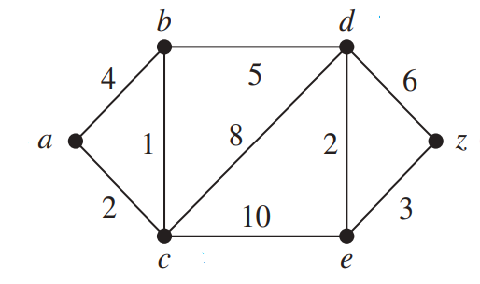
\includegraphics[height=3.7cm]{./img/lecture7-fig1.png}
  \end{center}
    
\end{frame}

\begin{frame}[plain]{}

  \begin{center}
     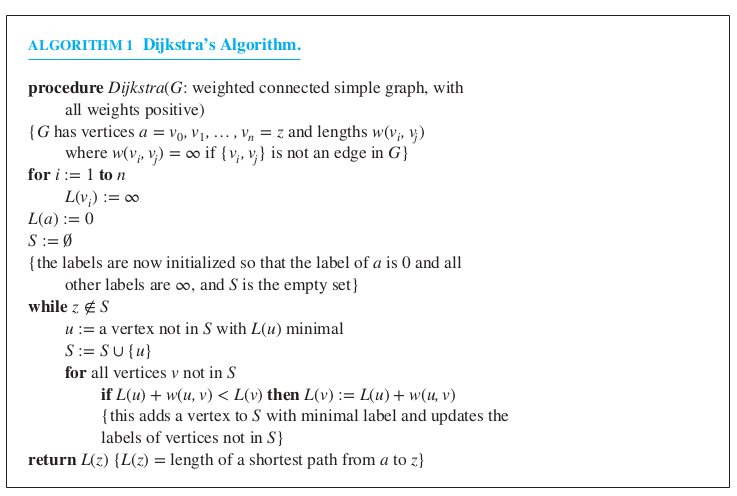
\includegraphics[height=8.5cm]{./img/lecture7-fig2.png}
  \end{center}
  
\end{frame}

\begin{frame}[plain]{}

 {\bf Visualization of Dijkstra's Algorithm:}
  \begin{center}
     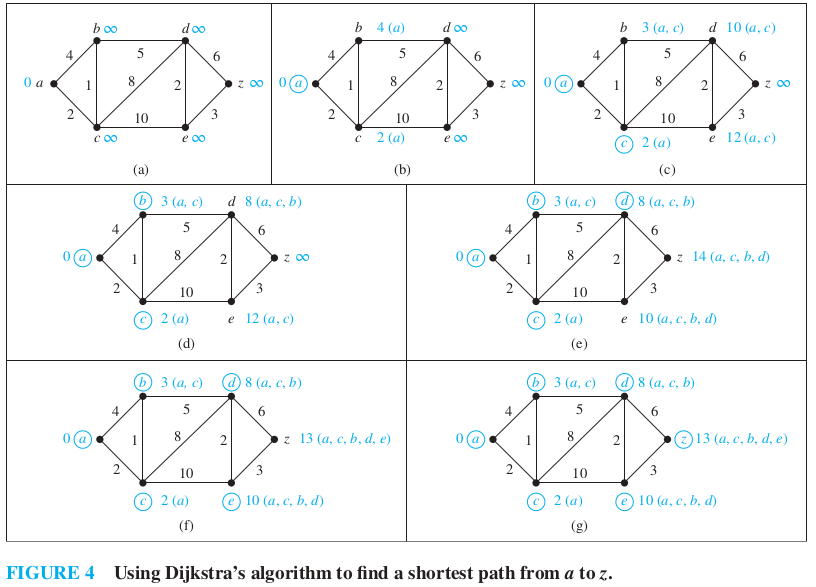
\includegraphics[height=8cm]{./img/lecture7-fig3.png}
  \end{center}
  
\end{frame}

\begin{frame}[plain]{}

{\bf Practice 7.2.} Use Dijkstra's algorithm to find a shortest path 
between $a$ and $z$ in the given weighted graph. Visualize the process as
Figure 4 on the previous slide.

 \begin{center}
     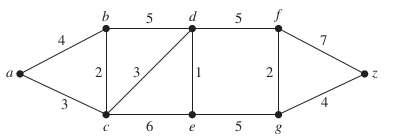
\includegraphics[height=3cm]{./img/lecture7-fig4.png}
  \end{center}
 
 \vspace{1in}
 
 {\bf Note:} It may be instructive to consider how Dijkstra's algorithm can be modified 
to find the shortest path in a non-simple graph.

\end{frame}

\begin{frame}[plain]{}
 
 Dijkstra's algorithm is fundamental in computer science and graph theory. 
 Understanding and learning to implement it opens doors to more advanced graph algorithms 
 and applications. %https://www.datacamp.com/tutorial/dijkstra-algorithm-in-python
 \medskip
 
 It also teaches a valuable problem-solving approach through 
 its {\bf greedy algorithm}, which involves making the optimal choice at each step based 
 on current information.
 \medskip
 
This skill is transferable to other optimization algorithms. 
Dijkstra’s algorithm may \Red{not be the most efficient} in all scenarios 
but it can be a good baseline when solving``shortest distance" problems.
 \medskip
 
Examples include:
\begin{itemize}
  \item GPS navigation systems finding the fastest route
  \item Routing data packets in computer networks
  \item Delivery services optimizing routes for efficiency
  \item Social networks (suggesting connections)
  \item Finance (finding optimal investment paths)
  \item Project management (finding the most efficient workflow)
\end{itemize}

\end{frame}


\begin{frame}[plain]{Dijkstra's algorithm and Ajacency Matrix}
  
 \begin{columns}[t] % contents are top vertically aligned
\begin{column}[c]{5cm}

  \begin{center}
      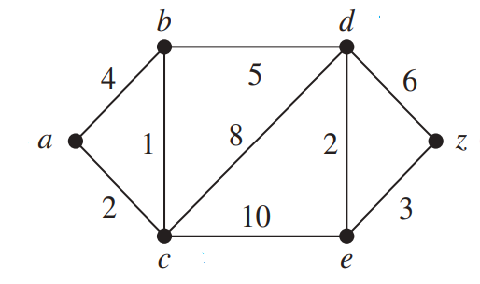
\includegraphics[height=3.7cm]{./img/lecture7-fig1.png}
  \end{center}
   
  \end{column} \pause
  \begin{column}[c]{5cm}
        \[ \mathrm{A}\ = \left[ \begin{array}{cccccc}
                            \Blue{0} & 4 & 2 & \Red{0} & \Red{0} & \Red{0} \\
                            4 & \Blue{0} & 1 & 5 & \Red{0} & \Red{0} \\
                            2 & 1 & \Blue{0} & 8 & 10 & \Red{0} \\
                            \Red{0} & 5 & 8 & \Blue{0} & 2 & 6 \\
                            \Red{0} & \Red{0} & 10 & 2 & \Blue{0} & 3 \\
                            \Red{0} & \Red{0} & \Red{0} & 6 & 3 & \Blue{0}
                           \end{array}
                    \right]                    
   \]   
  \end{column}
  \end{columns}

\end{frame}

\begin{frame}[plain]{ }
  %https://www.youtube.com/watch?v=Ww4nU_NcAIQ
  
 \begin{columns}[t] % contents are top vertically aligned
\begin{column}[c]{3.2cm}
{\small
  \[ \left[ \begin{array}{cccccc}
                            \Blue{0} & 4 & 2 & \Red{\infty} & \Red{\infty} & \Red{\infty} \\
                            4 & \Blue{0} & 1 & 5 & \Red{\infty} & \Red{\infty} \\
                            2 & 1 & \Blue{0} & 8 & 10 & \Red{\infty} \\
                            \Red{\infty} & 5 & 8 & \Blue{0} & 2 & 6 \\
                            \Red{\infty} & \Red{\infty} & 10 & 2 & \Blue{0} & 3 \\
                            \Red{\infty} & \Red{\infty} & \Red{\infty} & 6 & 3 & \Blue{0}
                           \end{array}
                    \right]                    
   \]   
}
   
  \end{column} 
  \begin{column}[c]{6.8cm}
     \begin{center}
         Distance from $a$
         \vspace{.2in}
         
       {\small  
        \begin{tabular}{ c|c||c|c|c|c|c|c}\hline
            Step &  Vertex & a & b & c & d & e & z \\ \hline
            \multirow{2}{*}{1}  & \onslide<2->  \multirow{2}{*}{a}  & \onslide<3-> 0a 
            & \onslide<4-> 4a
               & \onslide<5-> 2a & \onslide<6-> $\infty$  & \onslide<7-> $\infty$ 
                & \onslide<8-> $\infty$ \\ \cline{3-8}
              &   & \onslide<9-> $\cancel{0a}$  & 4a
               & \mycirc{2a} & $\infty$  & $\infty$ 
                & $\infty$ \\ \hline
                
            \onslide<10-> \multirow{2}{*}{2}  &   \multirow{2}{*}{c}  & \onslide<11-> $\cancel{0a}$ 
            & \onslide<12-> 3c
               & \onslide<13-> 2c & \onslide<14-> 10c  & \onslide<15-> 12c 
                & \onslide<16-> $\infty$ \\ \cline{3-8}
              &   & \onslide<17-> $\cancel{0a}$  & \mycirc{3c}
               & $\cancel{2c}$ & 10c  &  12c 
                & $\infty$ \\ \hline
                
            \onslide<18-> \multirow{2}{*}{3}  &  \multirow{2}{*}{b}  & \onslide<19-> $\cancel{0a}$ 
            & \onslide<20-> 3b
               & \onslide<21-> $\cancel{2c}$ & \onslide<22-> 8b  & \onslide<23-> 12c 
                & \onslide<24-> $\infty$ \\ \cline{3-8}
              &   & \onslide<25-> $\cancel{0a}$  & $\cancel{3b}$
               & $\cancel{2c}$ & \mycirc{8b}  & 12c 
                & $\infty$ \\ \hline 
                
             \onslide<26-> \multirow{2}{*}{4}  &  \multirow{2}{*}{d}  
              & \onslide<27-> $\cancel{0a}$ 
               &  $\cancel{3b}$
               & $\cancel{2c}$ & 8d  & \onslide<28-> 10d 
                & \onslide<29-> 14d \\ \cline{3-8}
              &   & \onslide<30-> $\cancel{0a}$  & $\cancel{3b}$
               & $\cancel{2c}$ &  $\cancel{8d}$  & \mycirc{10d}
                & 14d \\ \hline    
              
              \onslide<31-> \multirow{2}{*}{5}  &  \multirow{2}{*}{e}  
              & \onslide<32-> $\cancel{0a}$ 
               &  $\cancel{3b}$
               & $\cancel{2c}$ & $\cancel{8d}$  & \onslide<33-> 10e 
                & \onslide<33-> 13e \\ \cline{3-8}
              &   & \onslide<34-> $\cancel{0a}$  & $\cancel{3b}$
               & $\cancel{2c}$ &  $\cancel{8d}$  & $\cancel{10e}$
                & \mycirc{13e} \\ \hline                 
        \end{tabular}
        }
    \end{center} 
  \end{column}
  \end{columns}\pause
  \medskip
  
  Therefore, the shortest-path between a and z is ``\Blue{acbdez} of \Blue{length 13}."


%tikz example of generating graph and table 
% https://tex.stackexchange.com/questions/683781/automated-dijkstra-visualization

\end{frame}

\begin{frame}[plain]{Algorithm Complexity of Dijkstra’s algorithm = $\mathcal{O}(N^2)$}

When analyzing an algorithm for solving the shortest-path problem, 
we are interested in determining how much computational effort, or 'work,' 
the algorithm requires as a function of the number of vertices $N$ in the graph.
% which represents the problem's size. 
\pause
 Specifically, we aim to understand \Red{how the required work grows as 
 $N$ increases}. How much work does Dijkstra's algorithm require? \pause
 \begin{itemize}
   \item The set of all shortest routes is built up in $N$ steps, 
    by finding the closest node in Step 1, the next closest node in Step 2, and so on. \pause
   \item Each step requires examining the distance from the node that was “solved” 
   in the previous step to all unsolved nodes which can be reached from this node. \pause
   \item This requires examining at most $N-1$ edges in each of the $N$ steps,
    so the work required is $N (N-1) =  N^2-N$.\pause
   \item  We can be expressed the total work required by the algorithm 
     as a function of $N$ such as $\mathcal{O}(N^2)$. (We read $\mathcal{O}$
     as ``Big-O".)\pause
 \end{itemize}
 
 {\bf Interpretation:} An $\mathcal{O}(N^2)$ algorithm requires work that is proportional to $N^2$, 
 which means that doubling $N$ increases the work required by a factor of 4.
 (if $N=10\nearrow N=20$, then $10^2 \nearrow 20^2= 2^210^2 = 4 (10^2)$)

\end{frame}

\begin{frame}[plain]{}

 
 If an algorithm requires $\mathcal{O}(N^p)$ work for some $p$,
 then it is said to be a \Blue{polynomial time algorithm}.
 The larger $p$ is, the more rapidly the work grows with $N$. 
 Here are some examples of polynomial time
algorithms:
\begin{itemize}
 \item Finding the largest of $N$ values. Checking the value of each item and 
 keeping track of the largest value seen taken $\mathcal{O}(N)$ operations.
 \item Solving a system of $N$ linear equations in $N$ unknowns using 
  the Gaussian elimination algorithm takes $\mathcal{O}(N^3)$ operations.
  \item If the linear system is upper triangular, then it only takes $\mathcal{O}(N^2)$
   operations using ``back substitution".
  \item Dijkstra’s algorithm for finding the shortest path between two vertices in a network
 requires $\mathcal{O}(N^2)$. 
\end{itemize}

There are other problems which are essentially much harder, requiring
an amount of work which grows exponentially with the size of $N$, like $\mathcal{O}(2^n)$
or like $\mathcal{O}(N!)$. The \Blue{Traveling Salesman Problem (TSP)} is in this category. 

\end{frame}



\begin{frame}[plain]{ }

The \Blue{Traveling Salesman Problem (TSP)} 
 asks for an order in which a salesperson should visit each of the
cities on his route exactly once so that he travels the minimum total distance.
This is equivalent to
asking for a Hamilton circuit with minimum total weight 
in a complete graph, because each
vertex is visited exactly once in the circuit. 

\medskip

The most straightforward way to solve an instance of the TSP is
to examine all possible Hamilton circuits and select one of minimum total length.
How many circuits do we have to examine to solve the problem 
if there are $n$ vertices in the graph? 
Answer =  \Blue{$\frac{(n-1)!}{2} \approx \mathcal{O}(n^n)$}.
\medskip

Trying to solve a TSP in this way
 when there are only a few dozen vertices is impractical.
For example, with 25 verices, a total of $24!/2 \approx 3.1\times 10^{23}$
different Hamilton circuits would have to be considered.
\medskip

If it took just one nanosecond ($10^{-9}$) to examine each Hamilton
circuit, a total of approximately ten million years would be required 
to find a minimum-length
Hamilton circuit in this graph by exhaustive search techniques.


\medskip
While many algorithms have been developed which work very well
in practice, there is no algorithm known which is guaranteed to solve 
all TSP’s in less than exponential
time.


\end{frame}

 \end{document}

